\chapter{Resultados} \label{chap:resultados}
Aquí pondrán las gráficas que obtuvieron en la simulación de matlab para el robot (si las tienen), y las explicarán.

También mostrarán capturas de pantalla de cómo se ve en Gazebo el robot y en RViz, ya sea que funcione o no, para el cambio de trayectoria. Describirán lo que ocurre y por qué (si es que saben).

\subsubsection{Cinemática Directa}
\begin{figure}[H] 
	\centering
	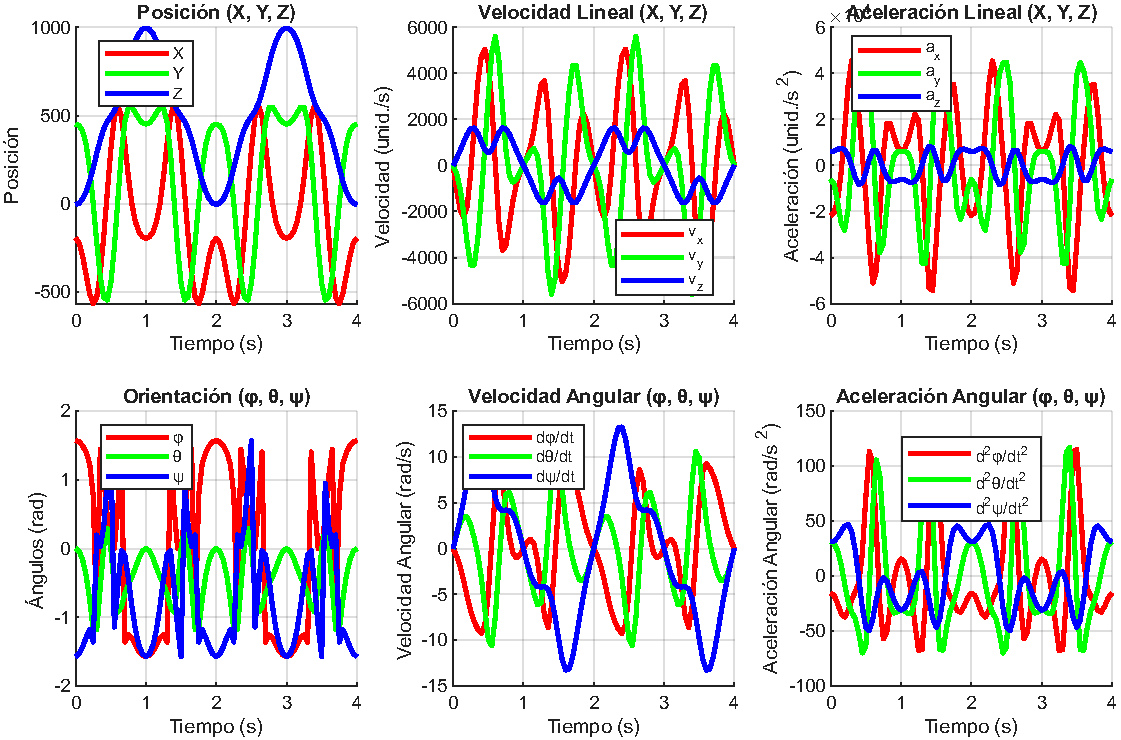
\includegraphics[width=0.8\textwidth]{Graficas_directa_robot_final.pdf}
	\caption{Gráficas cinemática directa en MATLAB.}
	\label{fig:TablasCinematicaDirecta}
\end{figure}

 
 El siguiente conjunto de gráficas representa el comportamiento cinemático de un robot, obtenido mediante la \textbf{cinemática directa} empleando los \textbf{parámetros de Denavit-Hartenberg (DH)}. Cada gráfico describe la evolución de diferentes variables en función del tiempo durante una trayectoria simulada.
 
 \begin{enumerate}
 	\item \textbf{Posición (X, Y, Z)} \\
 	\textit{Gráfica superior izquierda}
 	
 	Muestra la trayectoria espacial del extremo del robot en coordenadas cartesianas.
 	
 	El eje $X$ (rojo), $Y$ (verde) y $Z$ (azul) indican cómo varía la posición en cada uno de los tres ejes con el tiempo.
 	
 	\textbf{Interpretación}: el robot sigue una trayectoria oscilatoria en los tres ejes, lo que sugiere un movimiento complejo, posiblemente cíclico o programado con funciones senoidales o polinomiales.
 	
 	\item \textbf{Velocidad Lineal ($V_x$, $V_y$, $V_z$)} \\
 	\textit{Gráfica superior central}
 	
 	Representa la primera derivada temporal de la posición, es decir, cómo cambia la posición respecto al tiempo.
 	
 	Muestra la rapidez con la que el extremo del robot se mueve en cada dirección.
 	
 	\textbf{Interpretación}: se observa un comportamiento oscilatorio, indicando aceleraciones y desaceleraciones constantes. Las diferencias de amplitud entre ejes indican que el movimiento no es uniforme en todas las direcciones.
 	
 	\item \textbf{Aceleración Lineal ($a_x$, $a_y$, $a_z$)} \\
 	\textit{Gráfica superior derecha}
 	
 	Corresponde a la segunda derivada temporal de la posición.
 	
 	Informa sobre los cambios en la velocidad: aceleraciones positivas y negativas.
 	
 	\textbf{Interpretación}: los valores muestran picos bruscos y cambios rápidos, lo que sugiere que el robot experimenta variaciones rápidas en su movimiento, comunes en trayectorias con alta frecuencia de cambio o maniobras precisas.
 	
 	\item \textbf{Orientación ($\phi$, $\theta$, $\psi$)} \\
 	\textit{Gráfica inferior izquierda}
 	
 	Refleja la orientación del extremo del robot, típicamente representada en ángulos de Euler: roll ($\phi$ - rojo), pitch ($\theta$ - verde) y yaw ($\psi$ - azul).
 	
 	\textbf{Interpretación}: las oscilaciones indican que el robot cambia continuamente su orientación mientras sigue la trayectoria. La transición entre ángulos también sugiere rotaciones complejas, lo cual es habitual en brazos robóticos que deben mantener orientación específica.
 	
 	\item \textbf{Velocidad Angular ($\frac{d\phi}{dt}$, $\frac{d\theta}{dt}$, $\frac{d\psi}{dt}$)} \\
 	\textit{Gráfica inferior central}
 	
 	Representa la velocidad a la que cambian los ángulos de orientación.
 	
 	\textbf{Interpretación}: se identifican zonas de alta velocidad angular, lo que puede indicar maniobras de reorientación rápidas del efector final. El comportamiento es no uniforme y dependiente del ángulo específico.
 	
 	\item \textbf{Aceleración Angular ($\frac{d^2\phi}{dt^2}$, $\frac{d^2\theta}{dt^2}$, $\frac{d^2\psi}{dt^2}$)} \\
 	\textit{Gráfica inferior derecha}
 	
 	Es la segunda derivada de los ángulos respecto al tiempo, y describe cómo varía la velocidad angular.
 	
 	\textbf{Interpretación}: existen picos altos de aceleración angular, lo cual puede deberse a cambios bruscos de orientación en la trayectoria. Estos datos son importantes para evaluar el estrés dinámico sobre las articulaciones del robot.
 \end{enumerate}
 